\chapter{Neural Language Model (LM)}

\section{NN for NLP \cite{nlp-1}}

\begin{table}[H]
    \begin{minipage}{0.45\linewidth}
        \begin{figure}[H]
            \centering
            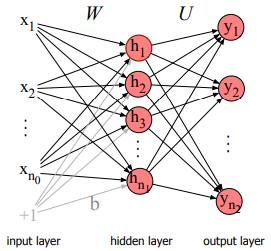
\includegraphics[height=6.5cm]{Pictures/nlp/simple-nn-nlp.png}
            \caption{Simple nn}
        \end{figure}
    \end{minipage}
    \hfill
    \begin{minipage}{0.45\linewidth}
        \begin{customTableWrapper}{1}
        \begin{table}[H]
            \begin{tabular}{l l l}
                 $\mathbf{x}$ & $[n_0, 1]$ & input vector \\
                 $\mathbf{h}$ & $[n_1, 1]$ & hidden layer \\
                 $\mathbf{h_i}$ &  & hidden unit \\
                 $\mathbf{W}$ & $[n_1, n_0]$ & weight matrix  ($x \rightarrow h$) \\
                 $\mathbf{W}_{ji}$ &  & weight ($x_i \rightarrow h_j$) \\
                 $\mathbf{b}$ & $[n_1, 1]$ & bias vector \\
                 $\sigma(\cdot)$ & & activation function \\
                 $\mathbf{y}$ & $[n_2, 1]$ & output vector \\
                 $\mathbf{U}$ & $[n_2, n_1]$ & weight matrix ($h \rightarrow z$) \\
                 $\mathbf{U}_{i,j}$ & & weight ($h_j \rightarrow z_i$) \\
                 $\mathbf{z}$ & $[n_2, 1]$ & intermediate output vector \\
            \end{tabular}
        \end{table}
        \end{customTableWrapper}
    \end{minipage}
\end{table}

\begin{table}[H]
    \begin{minipage}{3.5cm}
        \begin{enumerate}
            \item $\mathbf{h} = \sigma(\mathbf{W}\cdot \mathbf{x} + \mathbf{b})$
            \item $\mathbf{z} = \mathbf{U} \cdot \mathbf{h}$
            \item $\mathbf{y} = \operatorname{softmax}(\mathbf{z})$
        \end{enumerate}
    \end{minipage}
    \hfill
    \begin{minipage}{4.2cm}
        \begin{enumerate}
            \item $\mathbf{z}^{[1]} = \mathbf{W}^{[1]}\mathbf{a}^{[0]} +\mathbf{b}^{[1]}$
            \vspace{0.15cm}
            \item $\mathbf{a}^{[1]} = \mathbf{g}^{[1]}(\mathbf{z}^{[1]})$
            \vspace{0.15cm}
            \item $\mathbf{z}^{[2]} = \mathbf{W}^{[2]}\mathbf{a}^{[1]} +\mathbf{b}^{[2]}$
            \vspace{0.15cm}
            \item $\mathbf{a}^{[2]} = \mathbf{g}^{[2]}(\mathbf{z}^{[2]})$
            \vspace{0.15cm}
            \item $\mathbf{\hat{y}} = \mathbf{a}^{[2]}$
        \end{enumerate}
    \end{minipage}
    \hfill
    \begin{minipage}{6cm}
        \begin{algorithm}[H]
            \caption{Neural LM: n-layer Feed forward network}
            \For{\textit{i} \textbf{in} 1...n}{
                $\mathbf{z}^{[i]} = \mathbf{W}^{[i]}\mathbf{a}^{[i-1]} +\mathbf{b}^{[i]}$\;
                $\mathbf{a}^{[i]} = \mathbf{g}^{[i]}(\mathbf{z}^{[i]})$\;
            }
            
            $\mathbf{\hat{y}} = \mathbf{a}^{[n]}$\;
        \end{algorithm}
    \end{minipage}
\end{table}

\begin{figure}[H]
    \centering
    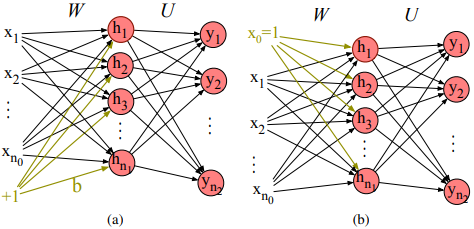
\includegraphics[height=4cm]{Pictures/nlp/neural-nn-replace_bias.png}
    \caption{Replacing the bias node (shown in a) with $x_0$ (b)}
\end{figure}

\section{Cross-entropy Loss ( $L_{CE}(\hat{\mathbf{y}},\mathbf{y})$ ) \cite{nlp-1}}

Logistic Regression Loss (Binary):
\[
    L_{CE}(\hat{y}, y) = -\log(p(y|x)) = -[y\cdot\log(\hat{y})+ (1-y)\cdot\log(1-\hat{y})]
\]

When number of classes $\geq 3$,
\begin{enumerate}
    \item $\mathbf{y}$ is vector = true labels
    \item $\mathbf{\hat{y}}$ is vector = predicted labels
\end{enumerate}

\vspace{0.3cm}
For class $k \in \dCurlyBrac{1,2,...,K}$ ($K$ classes),
\begin{enumerate}
    \item \(\mathbf{y_k} = \begin{cases}
        1 & \text{ if } \mathbf{y_k} = 1 \\
        0 & \text{ otherwise}
    \end{cases}\)
    \item One-hot vector $\mathbf{y} = [\mathbf{\hat{y}}_1, \mathbf{\hat{y}}_2, ..., \mathbf{\hat{y}}_K]$
    \item $\mathbf{\hat{y}}_k = p(\mathbf{y}_k = 1|\mathbf{x})$
\end{enumerate}

\vspace{0.2cm}
\[
    L_{CE}(\mathbf{\hat{y}}, \mathbf{y}) = -\sum_{k=1}^{K} \mathbf{y}_k\log(\mathbf{\hat{y}}_k)
\]
\begin{align*}
    L_{CE}(\mathbf{\hat{y}}, \mathbf{y}) &= -\sum_{k=1}^{K} \mathbbm{1}_{\mathbf{y}_k =1}\log(\mathbf{\hat{y}}_k) 
    \repeatn{16}{\quad} \text{(SEE: \fullref{Indicator function})}\\
    &= -\log(\mathbf{\hat{y}}_c) \repeatn{20}{\quad} \text{(where c is the correct class)}\\
    &= -\log\displaystyle\dfrac{\exp(\mathbf{z}_c)}{\sum_{j=1}^{K} \exp(\mathbf{z}_j)}  \repeatn{7}{\quad} \text{(using \fullref{Softmax function})}
\end{align*}


\subsection{Gradient of Loss}
\begin{align*}
    \dfrac{\partial L_{CE}(\mathbf{\hat{y}}, \mathbf{y})}{\partial w_j} &= (\hat{y} - y) \mathbf{x}_j \\
    &= (\sigma(\mathbf{w} \cdot \mathbf{x} + b) - y) \mathbf{x}_j
\end{align*}

\begin{align*}
    \dfrac{\partial L_{CE}(\mathbf{\hat{y}}, \mathbf{y})}{\partial \mathbf{w}_{k,i}} 
    &= -(\mathbf{y}_{k} - \mathbf{\hat{y}}_{k})\mathbf{x}_{i}\\
    &=-(\mathbf{y}_{k} - p(\mathbf{y}_{k}=1|\mathbf{x}))\mathbf{x}_{i}\\
    &=-\left(\mathbf{y}_{k} - \displaystyle\dfrac{\exp(\mathbf{w}_{k}\cdot \mathbf{x} + b_{k})}{\sum_{j=1}^{K} \exp(\mathbf{w}_{j}\cdot \mathbf{x} + b_{j})}\right)\mathbf{x}_i
\end{align*}

\section{Forward Inference (Decoding)}
Forward inference is the task, given an input, of running a forward pass on the network to produce a probability distribution over possible outputs, in this case next words.

\begin{enumerate}
    \item We first represent each of the $N$ previous words as a one-hot vector of length one-hot vector $\dabs{V}$, i.e., with one dimension for each word in the vocabulary.
    \item A \textbf{one-hot vector}\indexlabel{one-hot vector} is a vector that has one element equal to $1$ - in the dimension corresponding to that word’s index in the vocabulary - while all the other elements are set to $0$.
    \item Thus in a one-hot representation for the word “toothpaste”, supposing it is $V_5$, i.e., index $5$ in the vocabulary, $x_5 = 1$, and $x_i = 0 \quad\forall\quad i \neq 5$, as shown here:\\
    \begin{table}[h!]
        \centering
        \begin{tabular}{c c c c c c c c c}
            $0$ & $0$ & $0$ & $0$ & $1$ & $0$ & $0$ & ... & $0$\\
            $1$ & $2$ & $3$ & $4$ & $5$ & $6$ & $7$ & ... & $\dabs{V}$
        \end{tabular}
    \end{table}
\end{enumerate}

\begin{table}[H]
    \begin{minipage}{0.45\linewidth}
        \begin{figure}[H]
            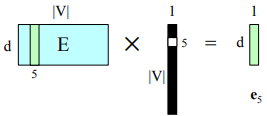
\includegraphics[width=\linewidth]{Pictures/nlp/fig-7-16.png}
            \caption{Selecting the embedding vector for word $V_5$ by multiplying the embedding matrix $E$ with a one-hot vector with a $1$ in index $5$}
        \end{figure}
    \end{minipage}
    \hfill
    \begin{minipage}{0.65\linewidth}
        \begin{enumerate}
            \item The feedforward neural language model has a \textbf{moving window} that can see $N$ words into the past.

            \item When $N=3$, so the $3$ words $w_{t-1}$, $w_{t-2}$, and $w_{t-3}$ are each represented as a one-hot vector.

            \item We then multiply these one-hot vectors by the \textbf{embedding matrix} \indexlabel{embedding matrix} $\mathbf{E}$.

            \item The \textbf{embedding weight matrix}\indexlabel{embedding weight matrix} $\mathbf{E}$ has a column for each word, each a column vector of $d$ dimensions, and hence has dimensionality $d \times \dabs{V}$. 
            
            \item Multiplying by a one-hot vector that has only one non-zero element $x_i = 1$ simply selects out the relevant column vector for word $i$, resulting in the embedding for word $i$.

            \item The 3 resulting embedding vectors are concatenated to produce $\mathbf{e}$, the embedding layer. 
            
            \item This is followed by a \textbf{hidden layer} and an output layer whose \textbf{softmax} produces a probability distribution over words.
        \end{enumerate}
    \end{minipage}
\end{table}
\begin{table}[H]
    \begin{minipage}{0.55\linewidth}
        \begin{figure}[H]
            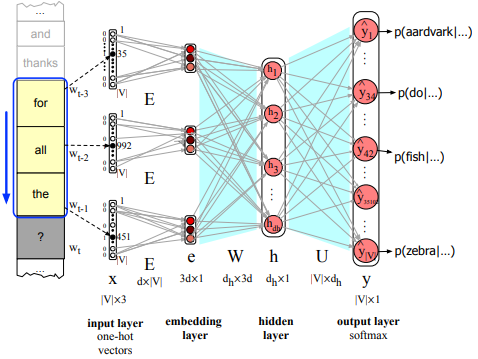
\includegraphics[width=\linewidth]{Pictures/nlp/fig-7-17.png}
            \caption{Forward inference in a feedforward neural language model}
        \end{figure}
    \end{minipage}
    \hfill
    \begin{minipage}{0.55\linewidth}
        \begin{enumerate}
            \item At each timestep $t$ the network computes a $d$-dimensional embedding for each context word (by multiplying a one-hot vector by the embedding matrix $E$), and concatenates the $3$ resulting embeddings to get the embedding layer $e$.
            
            \item The embedding vector $e$ is multiplied by a weight matrix $W$ and then an activation function is applied element-wise to produce the hidden layer $h$, which is then multiplied by another weight matrix $U$.

            \item Finally, a softmax output layer predicts at each node $i$ the probability that the next word wt will be vocabulary word $V_i$.
        \end{enumerate}
    \end{minipage}
\end{table}

\vspace{0.2cm}
Steps:
\begin{enumerate}
    \item \textbf{Select $3$ embeddings from} $\mathbf{E}$:\\
    Given the $3$ previous words, we look up their indices, create $3$ one-hot vectors, and then multiply each by the embedding matrix $\mathbf{E}$. The one-hot vector for word is multiplied by the embedding matrix $\mathbf{E}$, to give the first part of the first hidden layer, the \textbf{embedding layer}\indexlabel{embedding layer}. Since each column of the input matrix $\mathbf{E}$ is an embedding for a word, and the input is a one-hot column vector $x_i$ for word $V_i$, the embedding layer for input $w$ will be $Ex_i = e_i$, the embedding for word $i$. We now concatenate the 3 embeddings for the 3 context words to produce the embedding layer $\mathbf{e}$.
    \begin{center}
        \( \mathbf{e = [Ex_{t-3};Ex_{t-2};Ex_{t-1}]} \)
    \end{center}

    \item \textbf{Multiply by} $\mathbf{W}$: We multiply by $\mathbf{W}$ (and add $\mathbf{b}$) and pass through the ReLU (or other) activation function (SEE: \fullref{chapter: Activation Functions}) to get the hidden layer $\mathbf{h}$.
    \begin{center}
        \(\mathbf{h = \sigma(W\cdot e+b)}\)
    \end{center}

    \item \textbf{Multiply by U}:
    \begin{center}
        \(\mathbf{z = Uh}\)
    \end{center}

    \item \textbf{Apply softmax}: After the softmax, each node $i$ in the output layer estimates the probability $P(w_t=i|w_{t-1},w_{t-2},w_{t-3})$
    \begin{center}
        \(\mathbf{\hat{y} = \operatorname{softmax}(z)}\)
    \end{center}
    
\end{enumerate}

\subsection{Training}

\begin{customTableWrapper}{1}
\begin{table}[H]
    \begin{tabular}{|l|l|}
        \hline
         Trainable Parameters & \(\mathbf{\theta = E,W,U,b}\) \\
         \hline
         Loss & \( L_{CE}(\hat{y}, y) = -\log(\hat{y}_i) \) \\
         & \( L_{CE} = \log(p(w_t|w_{t-1},...,w_{t-n+1})) \) \\
         \hline
         SGD & \begin{minipage}{8cm}
             \vspace{0.2cm}
             \( \theta^{s+1} = \theta^s - \eta\displaystyle\dfrac{\partial[-\log(p(w_t|w_{t-1},...,w_{t-n+1}))]}{\partial\theta} \)
             \vspace{0.2cm}
         \end{minipage}\\
         \hline
    \end{tabular}
\end{table}
\end{customTableWrapper}































